
%%%%%%%%%%%%%%%%%%%%%%% file typeinst.tex %%%%%%%%%%%%%%%%%%%%%%%%%
%
% This is the LaTeX source for the instructions to authors using
% the LaTeX document class 'llncs.cls' for contributions to
% the Lecture Notes in Computer Sciences series.
% http://www.springer.com/lncs       Springer Heidelberg 2006/05/04
%
% It may be used as a template for your own input - copy it
% to a new file with a new name and use it as the basis
% for your article.
%
% NB: the document class 'llncs' has its own and detailed documentation, see
% ftp://ftp.springer.de/data/pubftp/pub/tex/latex/llncs/latex2e/llncsdoc.pdf
%
%%%%%%%%%%%%%%%%%%%%%%%%%%%%%%%%%%%%%%%%%%%%%%%%%%%%%%%%%%%%%%%%%%%


\documentclass[runningheads,a4paper]{llncs}

\usepackage{amssymb}
\setcounter{tocdepth}{3}
\usepackage{graphicx}
\usepackage{epstopdf}

\usepackage{url}
\urldef{\mailsa}\path|{up201305378, up201303501} @fe.up.pt |    
\urldef{\mailsb}\path| FEUP-PLOG, Turma 3MIEIC06, Grupo Akkoy_2 |
\newcommand{\keywords}[1]{\par\addvspace\baselineskip
\noindent\keywordname\enspace\ignorespaces#1}

\begin{document}

\mainmatter  % start of an individual contribution

% first the title is needed
\title{The use of restrictions in Logic Programming:\\Puzzle Akkoy}

% a short form should be given in case it is too long for the running head
\titlerunning{The use of restrictions in Logic Programming: Puzzle Akkoy}

% the name(s) of the author(s) follow(s) next
%
% NB: Chinese authors should write their first names(s) in front of
% their surnames. This ensures that the names appear correctly in
% the running heads and the author index.
%
\author{Filipa Ramos
\and Ines Santos}
%
\authorrunning{The use of restrictions in Logic Programming: Puzzle Akkoy}
% (feature abused for this document to repeat the title also on left hand pages)

% the affiliations are given next; don't give your e-mail address
% unless you accept that it will be published
\institute{Faculdade de Engenharia da Universidade do Porto,\\
Rua Dr. Roberto Frias, 4200 - 465, Porto, Portugal\\
\mailsa\\
\mailsb\\
\url{https://sigarra.up.pt/feup/pt/web_page.inicial}}

%
% NB: a more complex sample for affiliations and the mapping to the
% corresponding authors can be found in the file "llncs.dem"
% (search for the string "\mainmatter" where a contribution starts).
% "llncs.dem" accompanies the document class "llncs.cls".
%

\toctitle{The use of restrictions in Logic Programming}
\tocauthor{Puzzle Akkoy}
\maketitle


\begin{abstract}
The present report serves the purpose of explaning the process of finding a solution for akkoy puzzles using programming with restrictions. It also refers the implementation of restrictions in order to generate random puzzles. The main objective is to deepen the knowledge of \emph {PROLOG}, specially the clpfd library. The project was developed for the curricular unit of Logic Programming. The results will be evaluated in order to realize the efficiency of the found solution.
\keywords{restrictions programming logic prolog efficiency}
\end{abstract}


\section{Introduction}

This project was developed for the curricular unit of Logic Programming in order to deepen the knowledge of the clpfd prolog library. Between the many objectives accounted for this project, the following can be highlighted: examining the results of the use of restrictions whilst programming, understanding the logic of rule-based languages, realizing the advantages of logic in programming. The analized puzzle has many restrictions which made it hard to find a solution which incorporated all the restrictions. Besides this, the restrictions must be applied to different objects such as columns, rows and areas. The implemented solution uses the following approach: find out the different possibilities for each column and row according to the numbers given by the problem. The board that fills the restrictions in every row and column will be the solution. The returned board is a list of variables. Each number one represents a black square and each number zero represents a white square. 
The article is structured in order to make it easier to understand the solution. Firstly, the problem is described. Secondly, the solution and its visualization is explained. Finally, the results are analized and the conclusions are drawn. 

\section {Problem Description}

The presented problem consists in solving an akkoy puzzle. This puzzle has a blank board with numbers on the top and on the right. Figure \ref{example} represents a puzzle with size seven. 

\begin{figure}
\centering
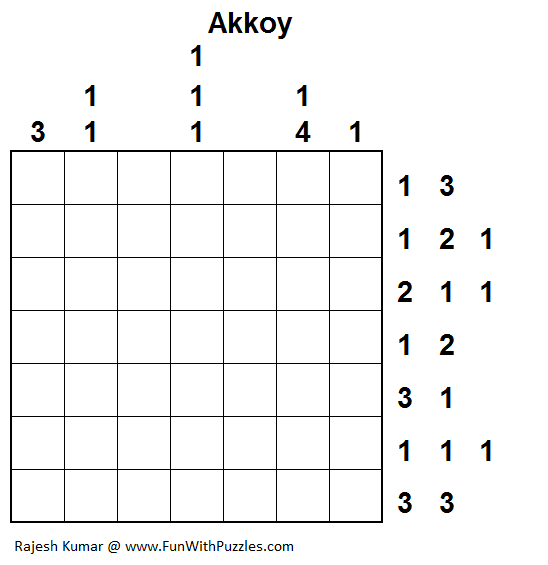
\includegraphics[height=6.2cm]{puzzleExemplo.png}
\caption{Example Puzzle.}
\label{example}
\end{figure}

The numbers on the top represent the number of black squares in each column. For example, in the fourth column there must be three black squares separated. The numbers on the right represent the number of white squares in each line. If these requirements are met, the solution will be a drawing composed of black and white areas (such as Figure \ref{solution}). 

\begin{figure}[h!]
\centering
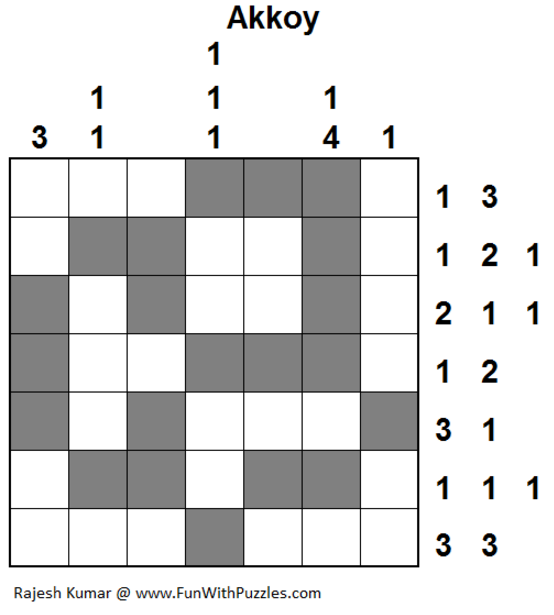
\includegraphics[height=6.2cm]{solucaoExemplo.png}
\caption{Solution of the example puzzle.}
\label{solution}
\end{figure}

If there are no numbers in a certain line or column it means that there are no restrictions on the respective line or column (restriction represented by [x]).

\section {Approach}

\subsection{Decision Variables}

	The following are the several decision variables used in the developed project: 
		\begin{enumerate}
			\item \verb|getPossibilities(S, Begins, R1)|
			\begin{enumerate}
				\item S represents the size of the row
				\item Begins are the decision variables
				\item R1 is the list with the restriction for the column
				\item domain is between 1 and S 
			\end{enumerate}
		\

			 - Returns a list with the possible index positions for areas in a row according to the given restrictions.
			The domain is from one to S because it represents all the possible positions on the row.

			 \item \verb|apply_restrictions(S, List, Restrictions, Color)|
			\begin{enumerate}
				\item S is the size of the row
				\item List is the row that is being restricted
				\item Restrictions is the list of the numbers for the respective row
				\item Color is the color that is being analized (white if it is a row/ black if it is a column)
				\item domain is between 0 and 1
			\end{enumerate}
		\

			- Restricts a single row. Domain is between black or white, 1 and 0 respectively.
	

			\item \verb|akkoy(Rcolumns, Rrows, Rows)|
				\begin{enumerate}
				\item Rcolumns is the list of lists of restrictions for each column
				\item Rrows is the list of lists of restrictions for each row
				\item Rows is the solved board
				\item domain is between 0 and 1
			\end{enumerate}
		\

			- Finds the solution for the problem by applying the restrictions.
		\end{enumerate}
		
\subsection{Constraints}

	The following constraints are applied:

	\begin{enumerate}
	\item \emph{List of numbers}
		- A number restriction is when there is a number or more on a column or row. These constraints are applied by \verb|apply_restrictions| which summons \verb|apply_merged| and \verb|apply_single_merged|. \verb|apply_restrictions| calls the other two until there are no more rows or columns to restrict. The two paint the cells in the right indexes (found with\verb|getPossibilities|) with the given color and paint the rest of the row the opposite color afterwards. 
	\item \emph{Empty list}
		- An empty list means there are no cells with that color on the row. If \verb|apply_restrictions| is called with an empty list of restrictions it calls \verb|swap_color| and \verb|color_all| which color the entire row with the opposite color.
	\item \emph{No restriction}
		- If a row has no restrictions any combination is possible. This is represented by [x]. If this happens, \verb|apply_restrictions| does not have any effect.
	\end{enumerate}

\subsection{Search Strategy}

	The labeling is called with an empty list of options (same as [leftmost,step,up,all]). This happens because of the problem which does not need any specific method to restrict the board.

\section{Solution Presentation}


\section{Results}


\section{Conclusions and Future Work}


\section{References}

\begin{thebibliography}{2}

\bibitem{url} Sicstus Prolog Manual, \url{https://www.kth.se/polopoly_fs/1.339598!/sicstus.pdf}

\bibitem{url} Clpfd Documentation, \url{https://sicstus.sics.se/sicstus/docs/4.1.0/html/sicstus/lib_002dclpfd.html}

\end{thebibliography}


\section{Annex}

\begin{equation}
  \psi (u) = \int_{o}^{T} \left[\frac{1}{2}
  \left(\Lambda_{o}^{-1} u,u\right) + N^{\ast} (-u)\right] dt \;  .
\end{equation}


\end{document}
